\section{Algorithm of the Shrinking aperture estimates}
\label{app:shrink_apert}
\begin{algorithm}
	\caption{Shrinking aperture algorithm with luminosity weights}
	\KwData{subhalo that satisfy cuts as a galaxy}
	 \hrulefill \\

	 initial aperture centroid = weighted mean galaxy location in each spatial dimension\\
 	distance array = euclidean distances between initial aperture center and each galaxy
	location \\
 	aperture radius = 90th percentile of the weighted distance array\\ 
	\While{ (newCenterDist - oldCenterDist) / oldCenterDist $\geq$ 2e-2}{
 		new data array = old data array within aperture\\
 		newCenter = weighted mean value of new data along each spatial dimension 
	}   \hrulefill
\end{algorithm}
\begin{figure*}
	\begin{center}
	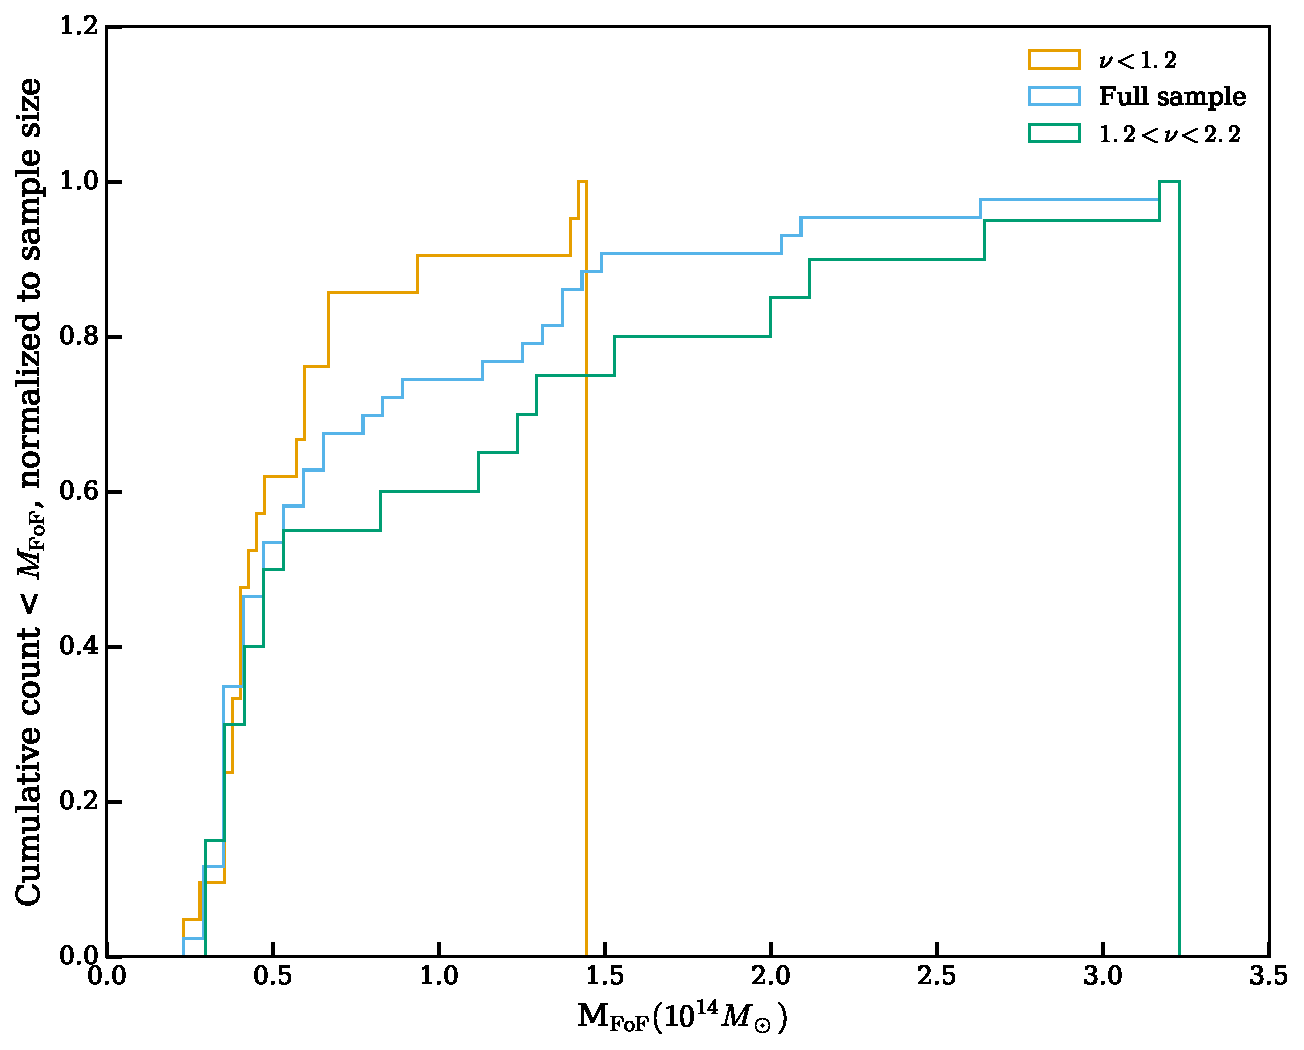
\includegraphics[width=0.7\linewidth]{Mass_abundance_relationship.pdf}
	\caption{Cumulative distribution of clusters above a certain mass threshold
		for different samples.
		Each distribution is normalized to the sample size.
		The unrelaxed samples $1.2 < \nu < 2.2$ 
		If the subsets have the same cluster mass abundance as the full sample,
		the three plots should lie on top of one another.
		\label{fig:mass_abundance_distribution}
	}
\end{center}
\end{figure*}
 

\section{Table of results}
\label{app:table_of_results}
\begin{landscape}
\begin{table}
	\begin{center}
	\caption{Properties of the clusters used in the analysis. Richness is
	computed based on $i-$band $< 24.4$ assuming $z=0.3$.\label{tab:cluster_prop}}
	\begin{tabular}{rrrrrrr}
\toprule
ID & richness & M$_{\rm 200C} (10^{14} M_\odot)$ & M$_{\rm 500C} (10^{14} M_\odot)$ & M$_{\rm FoF} (10^{14} M_\odot)$  & relaxedness$_0$ & relaxedness$_1$ \\
\midrule
 0 &      483 &                            16.35 &                            10.85 &                            32.29 &              29 &              33 \\
 1 &      338 &                            15.69 &                             6.16 &                            26.78 &              20 &              16 \\
 2 &      158 &                            15.33 &                             8.71 &                            21.20 &              17 &               3 \\
 3 &      134 &                             8.24 &                             5.63 &                            20.30 &              37 &              59 \\
 4 &      164 &                            11.93 &                             6.58 &                            15.42 &              21 &               4 \\
 5 &      115 &                             9.00 &                             5.65 &                            14.45 &              20 &              27 \\
 6 &       90 &                             9.58 &                             5.98 &                            14.01 &              18 &               7 \\
 7 &       92 &                             3.09 &                             1.74 &                            14.14 &              54 &             280 \\
 8 &      113 &                             8.25 &                             5.41 &                            13.36 &              24 &              26 \\
 9 &       97 &                             7.85 &                             4.98 &                            12.91 &              23 &              12 \\
10 &       83 &                             7.29 &                             5.33 &                            11.51 &              19 &               8 \\
11 &       86 &                             5.71 &                             3.32 &                             9.48 &              20 &               9 \\
12 &      267 &                             2.02 &                             0.87 &                             8.72 &              64 &             142 \\
13 &       84 &                             2.19 &                             1.43 &                             7.94 &              63 &             143 \\
14 &       89 &                             4.47 &                             2.88 &                             6.69 &              15 &               8 \\
15 &       70 &                             5.12 &                             3.50 &                             6.77 &              11 &               3 \\
16 &       68 &                             3.99 &                             2.30 &                             6.08 &              19 &               4 \\
17 &       66 &                             4.17 &                             1.84 &                             6.02 &              21 &               8 \\
18 &       79 &                             4.48 &                             3.15 &                             5.87 &              15 &               8 \\
19 &       61 &                             2.60 &                             1.85 &                             5.68 &              30 &              68 \\
20 &       69 &                             1.51 &                             1.08 &                             5.04 &              60 &             122 \\
21 &       62 &                             2.57 &                             1.23 &                             5.29 &              23 &               8 \\
22 &      343 &                             4.17 &                             3.05 &                             4.88 &              14 &               7 \\
23 &       59 &                             2.49 &                             1.72 &                             4.65 &              30 &              25 \\
24 &       57 &                             3.28 &                             2.62 &                             4.43 &              14 &              14 \\
25 &       56 &                             2.29 &                             1.50 &                             4.33 &              23 &              25 \\
26 &       69 &                             2.59 &                             1.81 &                             4.54 &              28 &              40 \\
28 &       63 &                             2.96 &                             1.64 &                             4.06 &              22 &              12 \\
29 &       69 &                             2.98 &                             2.05 &                             4.23 &              16 &              14 \\
30 &       72 &                             1.75 &                             1.36 &                             3.96 &              42 &              78 \\
31 &       63 &                             2.85 &                             2.12 &                             3.96 &              14 &              15 \\
32 &       55 &                             1.84 &                             1.29 &                             3.80 &              35 &              23 \\
33 &      213 &                             1.90 &                             1.03 &                             3.84 &              49 &              54 \\
34 &       54 &                             2.05 &                             1.41 &                             3.89 &              23 &              20 \\
35 &       52 &                             2.93 &                             2.17 &                             4.06 &              12 &               3 \\
36 &       53 &                             2.42 &                             1.62 &                             3.58 &              21 &              22 \\
37 &      212 &                             2.11 &                             1.55 &                             3.63 &              25 &              23 \\
39 &       56 &                             2.74 &                             1.79 &                             3.58 &              11 &               3 \\
40 &       58 &                             1.84 &                             0.99 &                             3.33 &              44 &              69 \\
46 &      225 &                             0.85 &                             0.58 &                             2.97 &              57 &              73 \\
48 &      230 &                             1.17 &                             0.85 &                             3.01 &              40 &             104 \\
51 &      148 &                             1.88 &                             1.34 &                             2.93 &              12 &               5 \\
58 &      187 &                             1.42 &                             0.88 &                             2.32 &              29 &              10 \\
\bottomrule
\end{tabular}

\end{center}
\end{table}
\end{landscape}

\begin{figure*}
	\begin{center}
	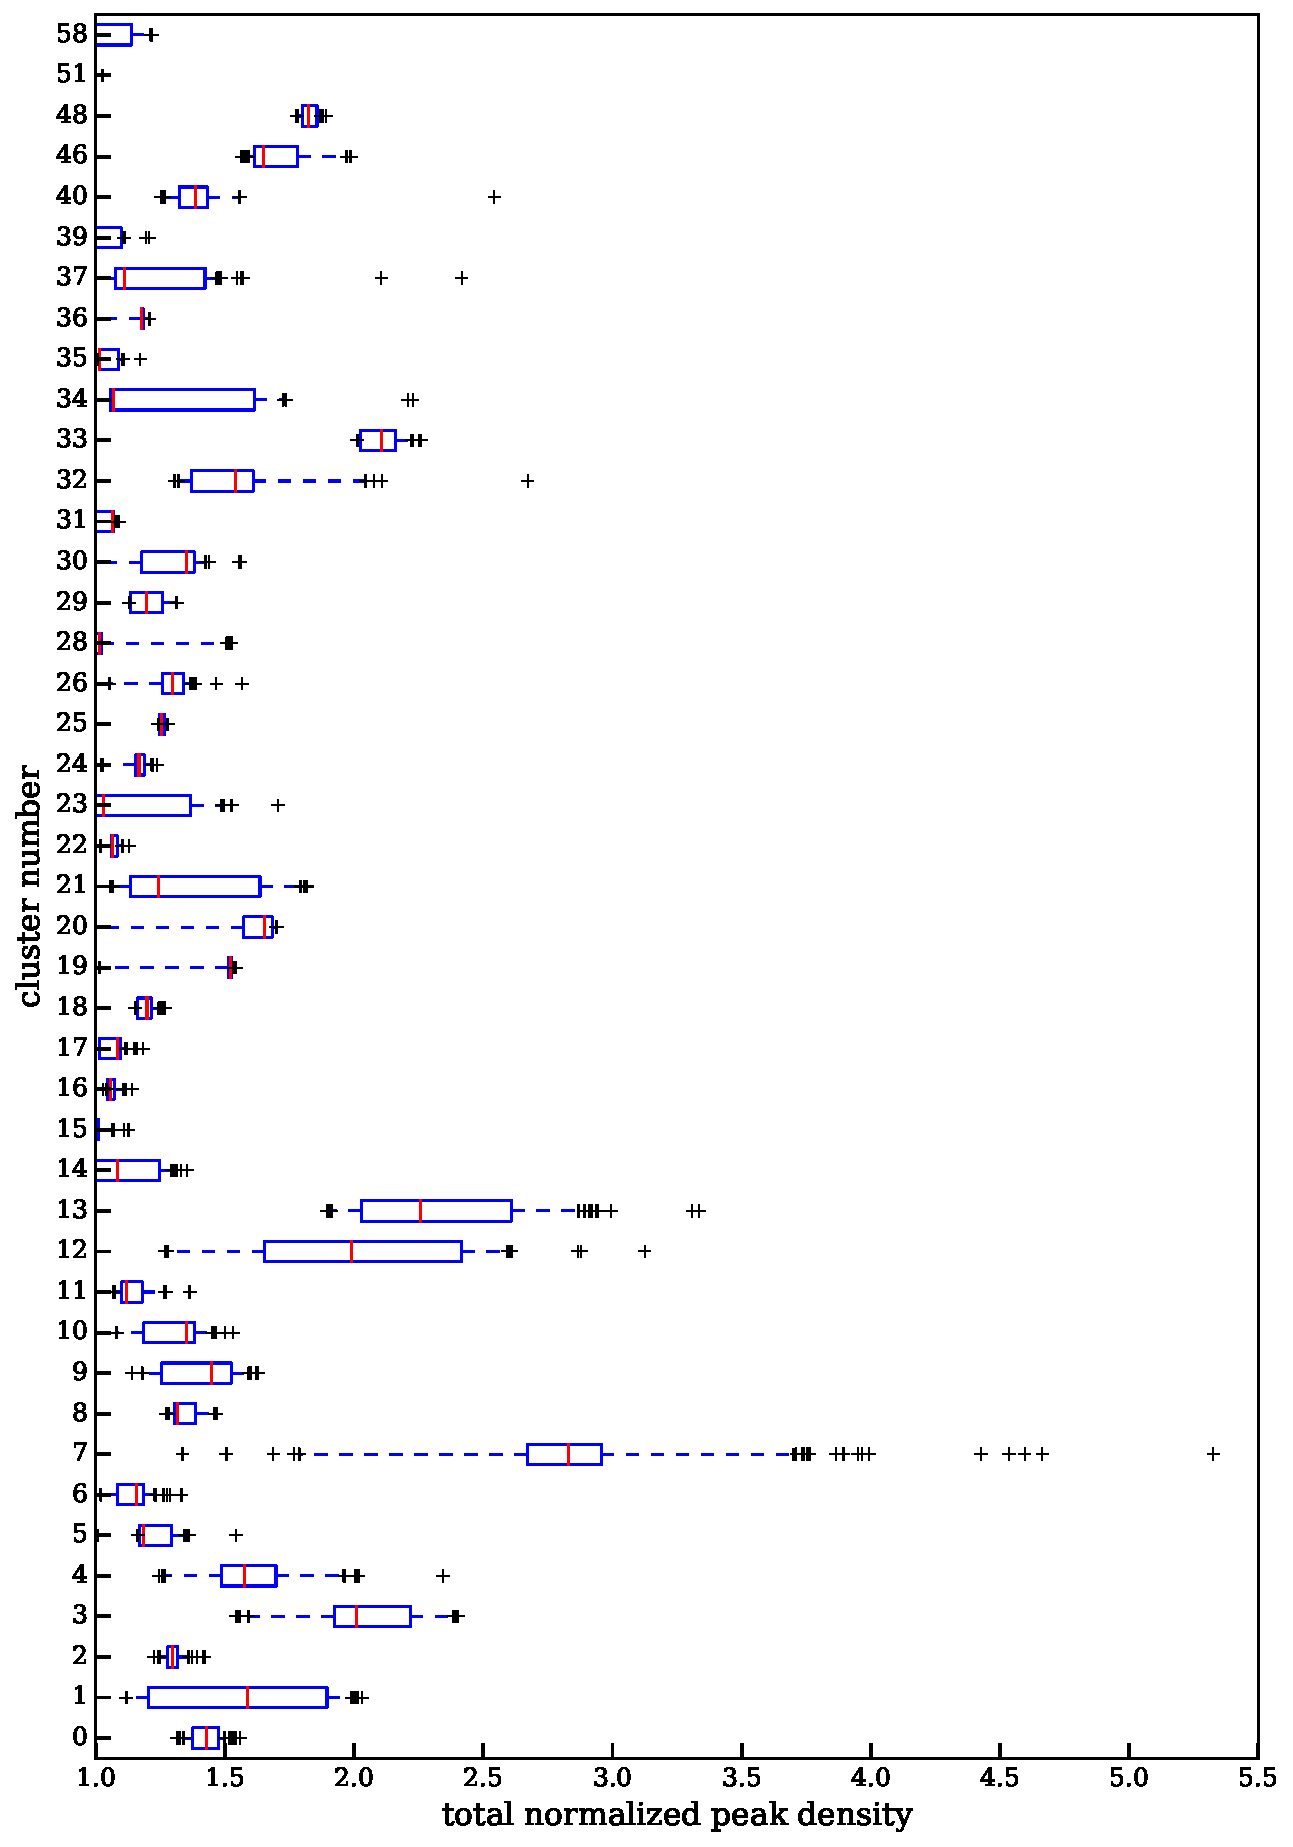
\includegraphics[width=0.85\linewidth]{fig8_total_normalized_peak_density.pdf}
	\caption{A box plot showing the distribution of the total normalized peak density 
		for each cluster 
		based on 768 projections. The red line shows the median of the projections,
		the box encompasses the 25\% and 75\% percentile of the distribution while
		the whiskers mark the 5\% and the 95\% percentile. The other black crosses
		are data points with extreme values beyond the 5\% and 95\% percentile.
		\label{fig:total_peak_dens_distribution}
	}
\end{center}
\end{figure*}


\begin{table*}
	\begin{center}
	\caption{Summary statistic characterizing the offset distributions
		between the most bound particle and various summary statistics of 
		the member galaxy population.
	\label{tab:most_bound_particle_offset_distributions}}
	\begin{tabular}{lrrrrrrr}
\toprule
{} &  location &  lower 68\% &  lower 95\% &  lower 99\% &  upper 68\% &  upper 95\% &  upper 99\% \\
\midrule
$\Delta y_{\rm BCG}$       &         0 &           -2 &          -2 &        -252
&          2 &         528 &        1107 \\
$\Delta y_{\rm centroid}'$ &         0 &        -134 &        -491 &       -1176 &         134 &         491 &        1176 \\
$\Delta y_{\rm KDE}'$      &         0 &         -19 &         -82 &       -1182 &          19 &          82 &        1182 \\
$\Delta y_{\rm num.dens}$  &         0 &         -83 &        -302 &       -1114 &          83 &         302 &        1114 \\
$\Delta y_{\rm shrink}'$   &         0 &         -50 &        -288 &       -1025 &          50 &         288 &        1025 \\
\bottomrule
\end{tabular}

\end{center}
\small{The offsets represented with the prime $'$ symbols are estimated using the luminosity weighted galaxy 
data.}
\end{table*}


\begin{table}
	\begin{center}
	\caption{Summary statistic characterizing the offset distributions
		for between the DM peak and the estimated galaxy location. 
		All 43 clusters and all 768 projections are used in this table. 
		The highest density values were used for the computation when there were more
		than one peak value estimated from the KDE.
	\label{tab:offset_distributions}}
	\begin{tabular}{lrrrrrrr}
\toprule
kpc &  mean &  std &   min &  25\% &  50\% &  75\% &  max \\
\midrule
$|\Delta s_{\rm BCG}|$       &    69 &  294 &     0 &    2 &    3 &    7 & 2335 \\
$\Delta x_{\rm BCG}$         &   -14 &  226 & -2331 &   -2 &   -0 &    1 & 2327 \\
$\Delta y_{\rm BCG}$         &    23 &  197 & -1980 &   -2 &    0 &    2 & 2332 \\
$|\Delta s_{\rm centroid}'|$ &   261 &  209 &     2 &  114 &  202 &  317 & 1103 \\
$\Delta x_{\rm centroid}'$   &   -42 &  224 & -1022 & -164 &  -37 &   66 & 1101 \\
$\Delta y_{\rm centroid}'$   &     0 &  244 & -1102 & -111 &   -0 &  111 & 1100 \\
$|\Delta s_{\rm shrink}'|$   &   118 &  156 &     0 &   21 &   60 &  165 & 1454 \\
$\Delta x_{\rm shrink}'$     &    -7 &  131 & -1089 &  -39 &   -3 &   23 &  969 \\
$\Delta y_{\rm shrink}'$     &     0 &  145 & -1091 &  -32 &    0 &   32 & 1109 \\
$|\Delta s_{\rm KDE}'|$      &    37 &   35 &     0 &   14 &   26 &   49 &  498 \\
$\Delta x_{\rm KDE}'$        &    -2 &   35 &  -330 &  -17 &   -2 &   12 &  386 \\
$\Delta y_{\rm KDE}'$        &    -0 &   37 &  -439 &  -15 &    0 &   15 &  440 \\
$\Delta s_{\rm num. KDE}$    &   136 &  161 &     1 &   56 &   92 &  147 & 2126 \\
$\Delta x_{\rm num. KDE}$    &   -12 &  142 & -1967 &  -55 &   -4 &   53 &  993 \\
$\Delta y_{\rm num. KDE}$    &    -0 &  155 & -1415 &  -54 &   -0 &   54 & 1417 \\
\bottomrule
\end{tabular}

\end{center}
\small{The offsets represented with the prime $'$ symbols are estimated using the luminosity weighted galaxy 
data.}
\end{table}




